% ============================================================================
% EXERCICES DU CHAPITRE
% Le fichier historique contient l'intégralité de la conversion Word.
% On n'exécute que la partie à partir de \section{Exercices du chapitre}.
% ============================================================================

\begingroup
\small
\sloppy
\setlength{\tabcolsep}{3pt}
\setlength{\LTleft}{0pt}
\setlength{\LTright}{0pt}
\setlength{\extrarowheight}{1pt}

% -----------------------------------------------------------------------------
% Images de l'ancienne conversion Word
% -----------------------------------------------------------------------------
\NewCommandCopy\TLLegacyIncludeGraphics\includegraphics

\NewDocumentCommand{\TLLegacyRawGraphic}{s O{} m}{%
  \ifstrempty{#2}{%
    \IfBooleanTF{#1}
      {\TLLegacyIncludeGraphics*[width=\linewidth,height=.82\textheight,keepaspectratio]{#3}}
      {\TLLegacyIncludeGraphics[width=\linewidth,height=.82\textheight,keepaspectratio]{#3}}%
  }{%
    \IfBooleanTF{#1}
      {\TLLegacyIncludeGraphics*[#2]{#3}}
      {\TLLegacyIncludeGraphics[#2]{#3}}%
  }%
}

\newcommand{\TLLegacyMissingGraphic}[1]{%
  \begin{tikzpicture}[baseline=(current bounding box.center)]
    \node[
      draw=TLCoverBlue!55,
      rounded corners=1mm,
      fill=TLCoverBlue!4,
      text=TLCoverBlue!80!black,
      align=center,
      font=\sffamily\scriptsize,
      inner sep=2mm,
      text width=24mm
    ] {Illustration vectorielle\\non convertie\\\ttfamily #1};
  \end{tikzpicture}%
}

\newcommand{\TLLegacyPlaceGraphic}[1]{%
  \ifinner
    \adjustbox{max width=.92\linewidth,max totalheight=.72\textheight}{#1}%
    \hspace{0pt}\allowbreak
  \else
    \par\noindent
    \makebox[\linewidth][c]{%
      \adjustbox{max width=.96\linewidth,max totalheight=.82\textheight}{#1}%
    }%
    \par\noindent
  \fi
}

\makeatletter
\RenewDocumentCommand{\includegraphics}{s O{} m}{%
  \begingroup
  \filename@parse{#3}%
  \edef\TLLegacyGraphicExtension{\filename@ext}%
  \edef\TLLegacyGraphicStem{\filename@area\filename@base}%

  \ifboolexpr{
    test {\ifstrequal{\TLLegacyGraphicExtension}{emf}}
    or test {\ifstrequal{\TLLegacyGraphicExtension}{EMF}}
    or test {\ifstrequal{\TLLegacyGraphicExtension}{wmf}}
    or test {\ifstrequal{\TLLegacyGraphicExtension}{WMF}}
  }{%
    \IfFileExists{\TLLegacyGraphicStem.png}{%
      \IfBooleanTF{#1}
        {\TLLegacyPlaceGraphic{\TLLegacyRawGraphic*[#2]{\TLLegacyGraphicStem.png}}}
        {\TLLegacyPlaceGraphic{\TLLegacyRawGraphic[#2]{\TLLegacyGraphicStem.png}}}%
    }{%
      \IfFileExists{\TLLegacyGraphicStem.pdf}{%
        \IfBooleanTF{#1}
          {\TLLegacyPlaceGraphic{\TLLegacyRawGraphic*[#2]{\TLLegacyGraphicStem.pdf}}}
          {\TLLegacyPlaceGraphic{\TLLegacyRawGraphic[#2]{\TLLegacyGraphicStem.pdf}}}%
      }{%
        \IfFileExists{\TLLegacyGraphicStem.jpeg}{%
          \IfBooleanTF{#1}
            {\TLLegacyPlaceGraphic{\TLLegacyRawGraphic*[#2]{\TLLegacyGraphicStem.jpeg}}}
            {\TLLegacyPlaceGraphic{\TLLegacyRawGraphic[#2]{\TLLegacyGraphicStem.jpeg}}}%
        }{%
          \IfFileExists{\TLLegacyGraphicStem.jpg}{%
            \IfBooleanTF{#1}
              {\TLLegacyPlaceGraphic{\TLLegacyRawGraphic*[#2]{\TLLegacyGraphicStem.jpg}}}
              {\TLLegacyPlaceGraphic{\TLLegacyRawGraphic[#2]{\TLLegacyGraphicStem.jpg}}}%
          }{%
            \TLLegacyPlaceGraphic{\TLLegacyMissingGraphic{\filename@base}}%
          }%
        }%
      }%
    }%
  }{%
    \IfBooleanTF{#1}
      {\TLLegacyPlaceGraphic{\TLLegacyRawGraphic*[#2]{#3}}}
      {\TLLegacyPlaceGraphic{\TLLegacyRawGraphic[#2]{#3}}}%
  }%
  \endgroup
}

\CatchFileDef{\TLLegacyModelisationFile}
  {02_ModelisationMecanismes_cours.tex}
  {}

% Les trois EMF ci-dessous se trouvent réellement dans la partie exercices.
% On les neutralise avant exécution du fichier capturé : pdfLaTeX ne voit donc
% jamais leur extension. image174 est une petite puce décorative ; les deux
% autres emplacements restent matérialisés par un repère discret.
\patchcmd{\TLLegacyModelisationFile}
  {
\includegraphics[width=\linewidth]{images/image174.emf}}
  {}
  {}{}
\patchcmd{\TLLegacyModelisationFile}
  {\protect
\includegraphics{images/image194.emf}}
  {\TLLegacyMissingGraphic{image194}}
  {}{}
\patchcmd{\TLLegacyModelisationFile}
  {
\includegraphics[width=\linewidth]{images/image220.emf}}
  {\TLLegacyMissingGraphic{image220}}
  {}{}

% Les images 158 et 159 étaient chacune demandées à \linewidth sur la même
% ligne. On les compose explicitement à 46 % de la largeur.
\patchcmd{\TLLegacyModelisationFile}
  {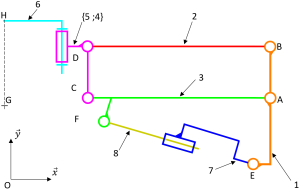
\includegraphics[width=\linewidth]{images/image158.png}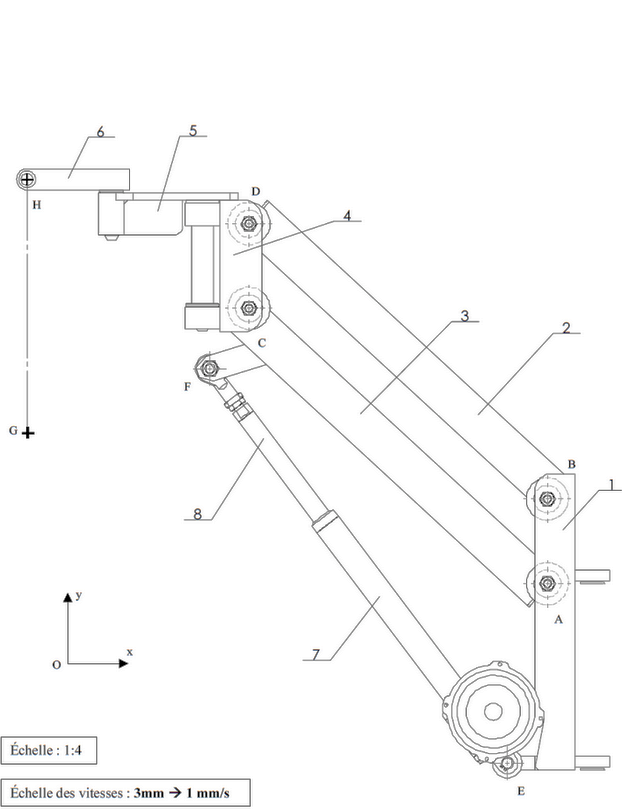
\includegraphics[width=\linewidth]{images/image159.png}}
  {\begin{center}%
   \TLLegacyIncludeGraphics[width=.46\linewidth]{images/image158.png}\hfill
   \TLLegacyIncludeGraphics[width=.46\linewidth]{images/image159.png}%
   \end{center}}
  {}{}

% Parcours récursif des commandes section du fichier capturé.
\long\def\TLExtractModelisationExercises#1\section#2#3\TLModelisationStop{%
  \ifstrequal{#2}{Exercices du chapitre}{%
    \section{#2}#3%
  }{%
    \expandafter\TLExtractModelisationExercises#3\TLModelisationStop
  }%
}

\expandafter\TLExtractModelisationExercises
  \TLLegacyModelisationFile
  \TLModelisationStop
\makeatother
\endgroup
